% Generated by Sphinx.
\def\sphinxdocclass{report}
\documentclass[letterpaper,10pt,english]{sphinxmanual}
\usepackage[utf8]{inputenc}
\DeclareUnicodeCharacter{00A0}{\nobreakspace}
\usepackage[T1]{fontenc}
\usepackage{babel}
\usepackage{times}
\usepackage[Bjarne]{fncychap}
\usepackage{longtable}
\usepackage{sphinx}
\usepackage{multirow}


\title{JWST Astronomy Data Analysis Tools Roadmap Documentation}
\date{August 12, 2013}
\release{0.1}
\author{Henry Ferguson, Perry Greenfield, and Alberto Conti}
\newcommand{\sphinxlogo}{}
\renewcommand{\releasename}{Release}
\makeindex

\makeatletter
\def\PYG@reset{\let\PYG@it=\relax \let\PYG@bf=\relax%
    \let\PYG@ul=\relax \let\PYG@tc=\relax%
    \let\PYG@bc=\relax \let\PYG@ff=\relax}
\def\PYG@tok#1{\csname PYG@tok@#1\endcsname}
\def\PYG@toks#1+{\ifx\relax#1\empty\else%
    \PYG@tok{#1}\expandafter\PYG@toks\fi}
\def\PYG@do#1{\PYG@bc{\PYG@tc{\PYG@ul{%
    \PYG@it{\PYG@bf{\PYG@ff{#1}}}}}}}
\def\PYG#1#2{\PYG@reset\PYG@toks#1+\relax+\PYG@do{#2}}

\expandafter\def\csname PYG@tok@gd\endcsname{\def\PYG@tc##1{\textcolor[rgb]{0.63,0.00,0.00}{##1}}}
\expandafter\def\csname PYG@tok@gu\endcsname{\let\PYG@bf=\textbf\def\PYG@tc##1{\textcolor[rgb]{0.50,0.00,0.50}{##1}}}
\expandafter\def\csname PYG@tok@gt\endcsname{\def\PYG@tc##1{\textcolor[rgb]{0.00,0.25,0.82}{##1}}}
\expandafter\def\csname PYG@tok@gs\endcsname{\let\PYG@bf=\textbf}
\expandafter\def\csname PYG@tok@gr\endcsname{\def\PYG@tc##1{\textcolor[rgb]{1.00,0.00,0.00}{##1}}}
\expandafter\def\csname PYG@tok@cm\endcsname{\let\PYG@it=\textit\def\PYG@tc##1{\textcolor[rgb]{0.25,0.50,0.56}{##1}}}
\expandafter\def\csname PYG@tok@vg\endcsname{\def\PYG@tc##1{\textcolor[rgb]{0.73,0.38,0.84}{##1}}}
\expandafter\def\csname PYG@tok@m\endcsname{\def\PYG@tc##1{\textcolor[rgb]{0.13,0.50,0.31}{##1}}}
\expandafter\def\csname PYG@tok@mh\endcsname{\def\PYG@tc##1{\textcolor[rgb]{0.13,0.50,0.31}{##1}}}
\expandafter\def\csname PYG@tok@cs\endcsname{\def\PYG@tc##1{\textcolor[rgb]{0.25,0.50,0.56}{##1}}\def\PYG@bc##1{\setlength{\fboxsep}{0pt}\colorbox[rgb]{1.00,0.94,0.94}{\strut ##1}}}
\expandafter\def\csname PYG@tok@ge\endcsname{\let\PYG@it=\textit}
\expandafter\def\csname PYG@tok@vc\endcsname{\def\PYG@tc##1{\textcolor[rgb]{0.73,0.38,0.84}{##1}}}
\expandafter\def\csname PYG@tok@il\endcsname{\def\PYG@tc##1{\textcolor[rgb]{0.13,0.50,0.31}{##1}}}
\expandafter\def\csname PYG@tok@go\endcsname{\def\PYG@tc##1{\textcolor[rgb]{0.19,0.19,0.19}{##1}}}
\expandafter\def\csname PYG@tok@cp\endcsname{\def\PYG@tc##1{\textcolor[rgb]{0.00,0.44,0.13}{##1}}}
\expandafter\def\csname PYG@tok@gi\endcsname{\def\PYG@tc##1{\textcolor[rgb]{0.00,0.63,0.00}{##1}}}
\expandafter\def\csname PYG@tok@gh\endcsname{\let\PYG@bf=\textbf\def\PYG@tc##1{\textcolor[rgb]{0.00,0.00,0.50}{##1}}}
\expandafter\def\csname PYG@tok@ni\endcsname{\let\PYG@bf=\textbf\def\PYG@tc##1{\textcolor[rgb]{0.84,0.33,0.22}{##1}}}
\expandafter\def\csname PYG@tok@nl\endcsname{\let\PYG@bf=\textbf\def\PYG@tc##1{\textcolor[rgb]{0.00,0.13,0.44}{##1}}}
\expandafter\def\csname PYG@tok@nn\endcsname{\let\PYG@bf=\textbf\def\PYG@tc##1{\textcolor[rgb]{0.05,0.52,0.71}{##1}}}
\expandafter\def\csname PYG@tok@no\endcsname{\def\PYG@tc##1{\textcolor[rgb]{0.38,0.68,0.84}{##1}}}
\expandafter\def\csname PYG@tok@na\endcsname{\def\PYG@tc##1{\textcolor[rgb]{0.25,0.44,0.63}{##1}}}
\expandafter\def\csname PYG@tok@nb\endcsname{\def\PYG@tc##1{\textcolor[rgb]{0.00,0.44,0.13}{##1}}}
\expandafter\def\csname PYG@tok@nc\endcsname{\let\PYG@bf=\textbf\def\PYG@tc##1{\textcolor[rgb]{0.05,0.52,0.71}{##1}}}
\expandafter\def\csname PYG@tok@nd\endcsname{\let\PYG@bf=\textbf\def\PYG@tc##1{\textcolor[rgb]{0.33,0.33,0.33}{##1}}}
\expandafter\def\csname PYG@tok@ne\endcsname{\def\PYG@tc##1{\textcolor[rgb]{0.00,0.44,0.13}{##1}}}
\expandafter\def\csname PYG@tok@nf\endcsname{\def\PYG@tc##1{\textcolor[rgb]{0.02,0.16,0.49}{##1}}}
\expandafter\def\csname PYG@tok@si\endcsname{\let\PYG@it=\textit\def\PYG@tc##1{\textcolor[rgb]{0.44,0.63,0.82}{##1}}}
\expandafter\def\csname PYG@tok@s2\endcsname{\def\PYG@tc##1{\textcolor[rgb]{0.25,0.44,0.63}{##1}}}
\expandafter\def\csname PYG@tok@vi\endcsname{\def\PYG@tc##1{\textcolor[rgb]{0.73,0.38,0.84}{##1}}}
\expandafter\def\csname PYG@tok@nt\endcsname{\let\PYG@bf=\textbf\def\PYG@tc##1{\textcolor[rgb]{0.02,0.16,0.45}{##1}}}
\expandafter\def\csname PYG@tok@nv\endcsname{\def\PYG@tc##1{\textcolor[rgb]{0.73,0.38,0.84}{##1}}}
\expandafter\def\csname PYG@tok@s1\endcsname{\def\PYG@tc##1{\textcolor[rgb]{0.25,0.44,0.63}{##1}}}
\expandafter\def\csname PYG@tok@gp\endcsname{\let\PYG@bf=\textbf\def\PYG@tc##1{\textcolor[rgb]{0.78,0.36,0.04}{##1}}}
\expandafter\def\csname PYG@tok@sh\endcsname{\def\PYG@tc##1{\textcolor[rgb]{0.25,0.44,0.63}{##1}}}
\expandafter\def\csname PYG@tok@ow\endcsname{\let\PYG@bf=\textbf\def\PYG@tc##1{\textcolor[rgb]{0.00,0.44,0.13}{##1}}}
\expandafter\def\csname PYG@tok@sx\endcsname{\def\PYG@tc##1{\textcolor[rgb]{0.78,0.36,0.04}{##1}}}
\expandafter\def\csname PYG@tok@bp\endcsname{\def\PYG@tc##1{\textcolor[rgb]{0.00,0.44,0.13}{##1}}}
\expandafter\def\csname PYG@tok@c1\endcsname{\let\PYG@it=\textit\def\PYG@tc##1{\textcolor[rgb]{0.25,0.50,0.56}{##1}}}
\expandafter\def\csname PYG@tok@kc\endcsname{\let\PYG@bf=\textbf\def\PYG@tc##1{\textcolor[rgb]{0.00,0.44,0.13}{##1}}}
\expandafter\def\csname PYG@tok@c\endcsname{\let\PYG@it=\textit\def\PYG@tc##1{\textcolor[rgb]{0.25,0.50,0.56}{##1}}}
\expandafter\def\csname PYG@tok@mf\endcsname{\def\PYG@tc##1{\textcolor[rgb]{0.13,0.50,0.31}{##1}}}
\expandafter\def\csname PYG@tok@err\endcsname{\def\PYG@bc##1{\setlength{\fboxsep}{0pt}\fcolorbox[rgb]{1.00,0.00,0.00}{1,1,1}{\strut ##1}}}
\expandafter\def\csname PYG@tok@kd\endcsname{\let\PYG@bf=\textbf\def\PYG@tc##1{\textcolor[rgb]{0.00,0.44,0.13}{##1}}}
\expandafter\def\csname PYG@tok@ss\endcsname{\def\PYG@tc##1{\textcolor[rgb]{0.32,0.47,0.09}{##1}}}
\expandafter\def\csname PYG@tok@sr\endcsname{\def\PYG@tc##1{\textcolor[rgb]{0.14,0.33,0.53}{##1}}}
\expandafter\def\csname PYG@tok@mo\endcsname{\def\PYG@tc##1{\textcolor[rgb]{0.13,0.50,0.31}{##1}}}
\expandafter\def\csname PYG@tok@mi\endcsname{\def\PYG@tc##1{\textcolor[rgb]{0.13,0.50,0.31}{##1}}}
\expandafter\def\csname PYG@tok@kn\endcsname{\let\PYG@bf=\textbf\def\PYG@tc##1{\textcolor[rgb]{0.00,0.44,0.13}{##1}}}
\expandafter\def\csname PYG@tok@o\endcsname{\def\PYG@tc##1{\textcolor[rgb]{0.40,0.40,0.40}{##1}}}
\expandafter\def\csname PYG@tok@kr\endcsname{\let\PYG@bf=\textbf\def\PYG@tc##1{\textcolor[rgb]{0.00,0.44,0.13}{##1}}}
\expandafter\def\csname PYG@tok@s\endcsname{\def\PYG@tc##1{\textcolor[rgb]{0.25,0.44,0.63}{##1}}}
\expandafter\def\csname PYG@tok@kp\endcsname{\def\PYG@tc##1{\textcolor[rgb]{0.00,0.44,0.13}{##1}}}
\expandafter\def\csname PYG@tok@w\endcsname{\def\PYG@tc##1{\textcolor[rgb]{0.73,0.73,0.73}{##1}}}
\expandafter\def\csname PYG@tok@kt\endcsname{\def\PYG@tc##1{\textcolor[rgb]{0.56,0.13,0.00}{##1}}}
\expandafter\def\csname PYG@tok@sc\endcsname{\def\PYG@tc##1{\textcolor[rgb]{0.25,0.44,0.63}{##1}}}
\expandafter\def\csname PYG@tok@sb\endcsname{\def\PYG@tc##1{\textcolor[rgb]{0.25,0.44,0.63}{##1}}}
\expandafter\def\csname PYG@tok@k\endcsname{\let\PYG@bf=\textbf\def\PYG@tc##1{\textcolor[rgb]{0.00,0.44,0.13}{##1}}}
\expandafter\def\csname PYG@tok@se\endcsname{\let\PYG@bf=\textbf\def\PYG@tc##1{\textcolor[rgb]{0.25,0.44,0.63}{##1}}}
\expandafter\def\csname PYG@tok@sd\endcsname{\let\PYG@it=\textit\def\PYG@tc##1{\textcolor[rgb]{0.25,0.44,0.63}{##1}}}

\def\PYGZbs{\char`\\}
\def\PYGZus{\char`\_}
\def\PYGZob{\char`\{}
\def\PYGZcb{\char`\}}
\def\PYGZca{\char`\^}
\def\PYGZam{\char`\&}
\def\PYGZlt{\char`\<}
\def\PYGZgt{\char`\>}
\def\PYGZsh{\char`\#}
\def\PYGZpc{\char`\%}
\def\PYGZdl{\char`\$}
\def\PYGZti{\char`\~}
% for compatibility with earlier versions
\def\PYGZat{@}
\def\PYGZlb{[}
\def\PYGZrb{]}
\makeatother

\begin{document}

\maketitle
\tableofcontents
\phantomsection\label{index::doc}

\begin{quote}\begin{description}
\item[{abstract}] \leavevmode\begin{quote}\begin{description}
\item[{author}] \leavevmode
Henry Ferguson, Perry Greenfield, and Alberto Conti

\item[{date}] \leavevmode
30 June 2013

\end{description}\end{quote}

The purpose of this document is to provide a roadmap for developing
the software tools that astronomers need for going from pipeline-reduced
data to scientific publications. The document looks at the process of
analyzing data for several different science cases, and looks at existing
tools in IRAF to identify the highest priorities for new tool development
or for porting of existing algorithms to a modern python environment.
For the most part, the numerical computations will be coded in Python and
incorporated into astropy. Many of the tools will have broad applicability
beyond JWST, so it makes sense for the code to be open source and the
development to be a broad community effort. This roadmap, while geared toward
JWST, is intended to foster a community dialog for the evolution of
these software tools.

\end{description}\end{quote}

Contents:


\chapter{Executive Summary}
\label{exec_summary:executive-summary}\label{exec_summary::doc}\label{exec_summary:jwst-astronomy-data-analysis-tools-roadmap}
This is a brief overview of the document.


\chapter{The vision}
\label{intro:the-vision}\label{intro::doc}
The overall vision of the data analysis tools effort is the following:
\begin{itemize}
\item {} 
To ensure that astronomers are equipped with software tools to analyze and interpret JWST data efficiently right from the start of the mission.

\item {} 
To reduce the necessity for astronomers to write data-analysis software.

\item {} 
To make it easier to do so when necessary.

\item {} 
To provide a rich set of modular software tools upn which to build

\item {} 
To make it easy to share \& re-use code.

\item {} 
To improve repeatability of scientific results.

\end{itemize}


\chapter{Guiding principles}
\label{intro:guiding-principles}
The following are guiding principles for developing this suite of software tools.
In this section, we describe both principle, the rationale for it, and the specific
choice that we have made (or are considering) to respond to that guiding principle.
Briefly, the guiding principles are:
\begin{enumerate}
\item {} 
Open source software

\item {} 
Easy to install

\item {} 
Well documented

\item {} 
Easy to extend

\item {} 
Multiple interfaces

\item {} 
Built on stable, widely adopted languages

\item {} 
Built on stable, widely adopted code libraries

\item {} 
Leverage existing codes and algorithms.

\end{enumerate}

These principles are by and large what distinguish
code intended to serve a broad community from code written by most individual
astronomers for their own day-to-day research.

We shall consider each principle in turn.


\section{Open Source Software}
\label{intro:open-source-software}
To ensure the repeatibility of modern scientific results, it is important that
the main computational code (not just the description of the algorithms) be
available to researchers. Repeatability should not mean re-investing hundreds of
man-years of effort to reproduce a chain of analysis, when the code could be
inspected and tested by independent researchers. Sometimes the error in a scientific
finding is not the result of a deep error of scientific judgment, but rather a
simple typo in computer code. \emph{The guiding principle for the Data Analysis Tools
is that all of the source code for the core numerical computations should be
open source.} It is less important that all of the code for GUI interfaces, image displays,
and interprocess communication be open source. Where practical, however, we will
adopt open-source solutions in preference to closed-source solutions.


\subsection{Licensing}
\label{intro:licensing}
There are a variety of \href{http://opensource.org/licenses}{open-source software licenses},
with various pros and cons.  The current plan is to adopt the 3-clause BSD-style license used for astropy.


\section{Easy to install}
\label{intro:easy-to-install}
With many astronomers having to do their own system administration, it
is important to make the software easy to install on the most commonly
used computing platforms.  This suggests the following high-level requirements:
\begin{enumerate}
\item {} 
A personal installation should be possible without system-administrator privileges

\item {} 
A multi-user shared installation should be possible with system-administrator privileges

\item {} 
The installation package should include all of the major library dependencies
\begin{enumerate}
\item {} 
The installation should not break or overwrite previously-installed versions of these libraries

\end{enumerate}

\item {} 
The software should have the ability to check if is up to date

\end{enumerate}

It is worth commenting that ease of installation does not preclude setting up
virtual machines, either on the user's own platform or in the cloud. Indeed,
if the installation procedure fulfills the goals above, setting up a virtual
machine would simply layer some steps on top to provide all of the OS and
programming-language infrastructure. While virtual machines are a very interesting
way of making computing available to the community, we do not envision that as
our primary method for providing access to the software.


\section{Well documented}
\label{intro:well-documented}
Excellent documentation is essential if the code is to fulfill the vision of being
easy to use, share, and extend.  The following are specific forms of documentation:
\begin{enumerate}
\item {} 
User guides

\item {} 
Cookbooks and tutorials

\item {} 
Help command or help buttons

\item {} 
Coding reference guide or API documentation

\item {} 
Comments in the source code

\end{enumerate}

In general, documentation should be available in the browser either on the web
or by pointing the browser to the local documentation repository, and the same
documentation should be available in pdf.  There have been significant advances
in the past 5 years in the ease of generating user and API documentation and
presenting it in multiple formats.  Our current plan is to use the
\href{http://sphinx-doc.org}{Sphinx} documentation generator to accomplish this.

The use of docstrings in python makes providing help easy, and the same text
is easily incorporated into the user guide. This is especially helpful for
the Application Programming Interface (API) documentation.

User guides provide a brief summary of each tool, describing the computational
algorithm and how to use it.  Tutorials and cookbooks provide worked examples,
often chaining together different tasks with discussion of the rationale behind
each step. Tutorials can be effective in the form of
\href{http://www.youtube.com/watch?v=DNRJwENqEUY}{videos}
or
\href{http://nbviewer.ipython.org/urls/raw.github.com/spacetelescope/scientific-python-training-2012/master/lecture\_notebooks/PSF\_Photometry\_Process.ipynb}{ipython notebooks}.


\section{Easy to extend}
\label{intro:easy-to-extend}
A typical workflow for an astronomer often starts with running a sequence
of tasks one-by-one on a specific data set, tuning the adjustable parameters
of each task to perfect the data processing. Once that is accomplished,
the astronomer will often want to chain these tasks together, possibly with
some extra code to set some of the parameters or follow some branch based on some property
of the specific data. It is extremely important that the tools be developed
in a way to facilitate this kind of work flow. This implies the following
goals for the data-analysis tools:
\begin{enumerate}
\item {} 
They should be modular

\item {} 
They should provide consistent APIs

\item {} 
They should provide easy-to-use libraries

\end{enumerate}

Being modular is somewhat hard to achieve. If the tasks are too primitive, then
there are too many steps needed to chain them together. If they are too complex,
then one ends up with a massive user guide to describe all of the adjustable
parameters or various kinds of I/O. An example of non-modular code (from the
perspective of most users) is the popular faint-galaxy photometry package
\href{http://www.astromatic.net/software/sextractor}{SExtractor},
which (for example) requires the user to re-run the source detection every time
one changes any input parameter even if the change has nothing to do with source
detection step. The user guide is excellent, and there is even an
excellent
\href{http://astroa.physics.metu.edu.tr/MANUALS/sextractor/Guide2source\_extractor.pdf}{SExtractor for dummies}
guide. But most astronomers won't get in and modify the code
itself because it is too intimidating. The C code itself is reasonably
modular, but the individual steps have not been exposed to be tweaked and
chained together in different ways. A more modular approach is exemplified
by the relatively new \href{http://scikit-image.org}{scikit-image}, which
provides a set of lower-level image-segmentation and image-morphology tasks
and a way to link then together in a pipeline.

The guiding principle for the JWST data analysis tools is to build
the complex tasks in a transparent,
well-documented way around the more primitive modules, and make it easy for
astronomers to modify a module or chain the modules together in a different way.

Providing consistent APIs means that modules that do similar things
should have a similar calling sequence. This is also somewhat hard
to achieve. Generally speaking it means adopting some common naming
conventions for parameters, and common method naming within classes
that have similar purposes.

If the code is modular and has consistent APIs, then providing easy-to-use
libraries means packaging the different modules in a sensible way
and providing good documentation. This is also somewhat of a challenge
to achieve, especially if the libraries incorporate community-generated
code.


\section{Multiple interfaces}
\label{intro:multiple-interfaces}
In developing the data analysis tools, a guiding principle is that
the basic numerical algorithms should be available through multiple
interfaces:
\begin{enumerate}
\item {} 
Via the command line

\item {} 
Via a scripting interface

\end{enumerate}

And that the scripting interface should support calling the
same routines from:
\begin{enumerate}
\item {} 
Various GUI interfaces

\item {} 
Client-server interfaces

\end{enumerate}

Most astronomers are comfortable working with tasks at the command-line
level (even if that command line is within an environment like IRAF or IDL).
Most astronomers are also accustomed to chaining tasks together
in a scripting language. The software will use python as the scripting language.

As the number of parameters grows or the level of interactivity grows, it is
important to have graphical user interfaces (GUIs). These usually interact
with other processes via events, and event-handlers which trigger calls to
a specific subroutine. A goal for the JWST data analysis tools is to segregate
the numerical computations from the GUI so that multiple GUIs can access
the same code, and so that the same code that is feeding the GUIs can be used
by astronomers in their scripts. (This was not the case, for example, with
the Java-based HST Exposure Time Calculators.) The challenge to enabling
multiple GUIs is to develop a well-documented GUI abstraction layer.

It is becoming increasingly common for astronomers or astronomical institutions
to provide web services that involve some computation. A goal is to make
it easy to use the data analysis tools to build such services on the \emph{server side}.
This should be straightforward.

It is \emph{not} a goal make the numerical-computation portion of the software compatible
with client-side computing in the browser. Most of the computations are too
complex for this to be practical, and the numerical libraries to support this
are generally lacking. However, the concept of developing GUIs within the browser
is very appealing.


\section{Stable, widely adopted languages}
\label{intro:stable-widely-adopted-languages}
There is a strong tension between the desire for a stable computing
platforming and the desire for a platform that incorporates
the latest cutting-edge computational developments. This roadmap aims for
a happy medium by choosing languages that are widely used
in science -- not just astronomy -- and are also widely used outside
of the sciences.
\begin{enumerate}
\item {} 
C

\item {} 
Python

\item {} 
Javascript (for browser interfaces but not for heavy numerical computation)

\end{enumerate}

All three languages are in the top 10 of
the \href{http://www.tiobe.com/index.php/content/paperinfo/tpci/index.html}{TIOBE index} of programming
language popularity and are considered mainstream. All three are very popular
outside of science based on metrics such as the number \href{http://jobstractor.com/monthly-stats}{job advertisements}  or
\href{https://sites.google.com/site/pydatalog/pypl/PyPL-PopularitY-of-Programming-Language}{searches for language tutorials},
popularity on
\href{http://redmonk.com/sogrady/2013/02/28/language-rankings-1-13/}{GITHub and Stack Overflow},
or popularity in a
\href{http://langpop.com}{variety of other metrics}. This is not to say these languages
are better or worse than others, simply that they are safe choices and are likely
to have a large developer community for at least the next decade.  In contrast,
the scripting languages used by R, IRAF, IDL, and MATLAB are unique to those environments,
making for a smaller communities of software developers, less open-source code, and
less community-based online support.

The general strategy will be to code as much as possible in Python,
moving to C when it offers significant performances advantages, and using
Javascript only for browser interfaces.


\section{Stable, widely adopted libraries}
\label{intro:stable-widely-adopted-libraries}
The numerical and scientific libraries available for Python and C
are substantial. For python, the code will leverage the many developer-years
invested in the following packages:
\begin{enumerate}
\item {} 
numpy -- The standard python array-manipulation package

\item {} 
scipy -- Scientific, numerical and statistical libraries

\item {} 
matplotlib -- 2-D (and some 3D) graphics

\item {} 
astropy -- Astronomy-oriented tasks

\item {} 
ipython and ipython notebook -- user interfaces

\item {} 
ConfigObj -- configuration file handling

\end{enumerate}
\begin{description}
\item[{For C, we plan to adopt the following libraries:}] \leavevmode\begin{enumerate}
\item {} 
CFITSIO?

\item {} 
What else?

\end{enumerate}

\end{description}

There are a variety of other libraries under development, which may or may not
be useful for the Astronomy Tools development. These will be discussed under Technologies and
Infrastructure.

We expect that many if not most of the Data Analysis tools developed in
this roadmap will be part of astropy.


\section{Leverage existing codes \& algorithms}
\label{intro:leverage-existing-codes-algorithms}
Where practical, we will re-use existing code or algorithms. For IDL and IRAF,
this generally means trying to draw from the algorithms rather than the code.
For python code, the general strategy will be to try to get it incorporated
into astropy and up to the astropy standards for configuration control and
documentation.


\chapter{Why do we need new tools?}
\label{intro:why-do-we-need-new-tools}
There are a variety of reasons why a development effort is needed for data
analysis tools for JWST. First and foremost, it is important to reduce the
amount of time between receipt of the data and achieving the scientific result.
Shortening this cycle is incredibly important because of JWST's limited lifetime.


\section{Make science more efficient}
\label{intro:make-science-more-efficient}
Most astronomers spend large amounts of time writing computer code (usually
scripts) to manipulate, view, and analyze data. A set of modern, well-documented
tools can reduce this coding burden and speed up the process of converting data into
scientific knowledge.  If a piece of code is re-used by more than one
astronomer, there is savings of a factor of two in development
cost per astronomer-hour, minus the time spent training the second astronomer
in how to use the code. Since the funding for astronomers and science-software
development come from the same source, this is an instant savings, and basically
translates to more science per dollar. The data-analysis tools described
here will be useful to hundreds of astronomers, so even counting time spent
writing documentation and training people in the use, the investment will
be worthwhile -- provided that the tools are actually tools that astronomers
want to use (hence the importance of community engagement in their development).

Third, there are specific
tools that are either non-existent in the community, or nowhere near at
the state of maturity needed for JWST --
e.g. tools for support of 3D spectroscopy, tools for dealing with JWST
error arrays and WCS information, tools for simulating JWST data, and
tools for simultaneously using data from HST, JWST, ALMA, and other facilities
in a seamless and statistically rigorous fashion.


\section{Remove scientist dependency on IRAF}
\label{intro:remove-scientist-dependency-on-iraf}
It  is widely recognized that continuing to develop
software based on core IRAF libraries, which are largely written in SPP and CL,
two languages that have no community outside of IRAF, would be inefficient
and costly in the long run. We need a graceful way to retire CL, SPP, and
dependencies on core IRAF.  (The extensive set of high-level analysis tools
written in SPP, together with the relatively large number of astronomers that
still use the CL for IRAF scripting make this a challenge.)

In a sense, the astronomical community is encumbered with a
technical debt in IRAF. Forcing the JWST scientific community to
rely on that platform for day-to-day their data analysis and visualization coding
makes no long-term economic sense.
Indeed, IRAF core development has been starved of resources over the
past few years, making it even more obsolete relative to other
options. Paying down the debt requires investment (in real dollars, or
FTE), but will pay off in the long run in greater science efficiency.

STScI developed PyRAF as a step in this evolution. Pyraf brought more powerful
scripting, error handling, and array-manipulation capabilities, better interoperability
with other languages, and access to a growing body of open-source scientific libraries.
Partly as a result of this, a growing fraction of astronomers entering the field
are using the python language as a central part of their software toolbox. For
that generation, the transition away from IRAF entirely should be relatively
painless once some of the core functionality is replaced.


\section{Modern programming language}
\label{intro:modern-programming-language}
Programming languages continue to evolve. Modern languages have
evolved to keep up with changes in computer architectures and changes
in coding paradigms. Choosing popular languages like C and Python helps
ensure that the language will keep up with the changes in computer
hardware. For IRAF, the burden of making those underlying changes falls
entirely on the astronomical community, for IDL or MATLAB it largely falls on a
single corporation with its own strategic goals.

Python in particular offers the following modern features, which make
it particularly attractive for writing most of the code:
\begin{itemize}
\item {} 
It is a high-level, interpreted language

\item {} 
It has a clean, readable syntax

\item {} 
It is very portable

\item {} 
It supports both object-oriented programming, and procedure-oriented programming

\item {} 
It supports 64-bit architectures and threading multiple CPUs

\item {} 
It has extensive error handling capabilities

\item {} 
It is free and open source

\item {} 
It can be extended with other languages (e.g. C)

\end{itemize}

The main practical advantage relative to the IRAF CL is that it is possible
to do efficient array arithmetic like in IDL and MATLAB, and there are extensive libraries
to support scientific computations. Another significant advantage is Python's
error trapping, which makes debugging code much easier than for the CL.
The advantages relative to IDL, Matlab, and R are primarily the language syntax,
its popularity, and the fact that it is free. In terms of speed for most
numerical computations Python+numpy is comparable to IDL and Matlab --
faster for some operations, slower for others.

Python takes about 1/6 the number of lines of code as C, which at least
anecdotally translates into a significant decrease in the amount of time
it takes an experience programmer to write their program. Since coding
is Python is relatively quick, one can develop the functionality in Python
first and address any performance bottlenecks on the second iteration.

The downside of adopting a state-of-the-art language, of course, is that it is evolving.
There is an ongoing cost for code maintenance to handle compatibility problems
as the languages evolve.


\section{Make better use of community code}
\label{intro:make-better-use-of-community-code}
The overall cost of data analysis tool development could be reduced
if there were more sharing and less duplication of effort. Therefore
an important part of building a new analysis-tool infrastructure is
to encourage such code sharing. This has become more common and
easier now with the rise in popularity of tools like \href{https://github.com}{github} for
open-source development.  Astropy includes
\href{http://www.astropy.org/affiliated/}{afffilated packages}
that are not part of the core source code but can be found
from the astropy website. Astropy does not depend on these packages,
but the packages may depend on astropy. These must be downloaded and
installed separately from astropy itself.

Strategies that can help encourage sharing of community code include
providing:
\begin{itemize}
\item {} 
Rubust, well-documented libraries in upon which to build.

\item {} 
Easy-to-follow standards for source-code style and documentation.

\item {} 
Templates for source code.

\item {} 
Clear instructions on how to package the code so that it can be installed on multiple platforms, along with expert assistance when necessary or feasible.

\item {} 
An active developers' forum.

\end{itemize}


\section{Modern algorithms where relevant}
\label{intro:modern-algorithms-where-relevant}
There has been considerable evolution over the past few decades
in the techniques and algorithms used to analyze data, not only in
astronomy but also in other fields. This includes advances in
statistical techniques such as resampling and Monte-Carlo
Markov Chains (MCMC), different ways  to approach the challenges
of model fitting or optimization (e.g. genetic algorithms), and
different ways to compress or describe data via basis functions
(e.g. wavelets, shapelets, Karhunen-Loeve decompositions, etc.).
Implementations of many of these exist already in the python/C
ecosystem, so including them in the astronomer's toolbox in many
cases may just be an issue of documentation and packaging.


\section{Leverage advances in computer hardware}
\label{intro:leverage-advances-in-computer-hardware}
Computer hardware has evolved significantly since IRAF was
developed. A significant fraction of the IRAF infrastructure,
for example, deals with operating-system abstraction (allowing
inter-operability with VAX/VMS and Unix) with network abstraction,
and with magnetic tape I/O. In the meantime, standard desktop and laptop
computer hardware now
offers featuers such as full 64-bit addressing, multiple cores,
hardware graphics acceleration and computation in graphics
processing units (GPUs).  A lot of infrastructure for using these
hardware advances already exists for Python and C, although
some of it is evolving rapidly (e.g. for GPUs).

Section {\color{red}\bfseries{}**}* discusses this infrastructure in more detail, with
an indication of which current libraries and packages are under
consideration.


\chapter{Science Use Cases}
\label{use_cases::doc}\label{use_cases:science-use-cases}
This section of the roadmap provides examples of the analysis flow
for different types of JWST science. These flow diagrams start where the
JWST pipeline leaves off. The data have been calibrated, rectified, co-added,
and extracted according to the standard pipeline algorithms. We assume
that these calibrations are sufficient, or that the astronomer can re-run
the pipeline if needed. The steps shown here are much more difficult to support
in a general-purpose pipeline, because they often depend on the specific science
goals and require inspection and judgement from the investigator at various
steps. They may also combine data from other missions, which is beyond
the scope of the JWST pipeline.

The flow diagrams shown here are not meant to be exhaustive or definitive.
They are illustrations of the flow that astronomers would expect to follow
if they received JWST data today.


\section{Faint Galaxies}
\label{use_cases:faint-galaxies}
Here is a flow diagram.
\begin{figure}[htbp]
\centering
\capstart

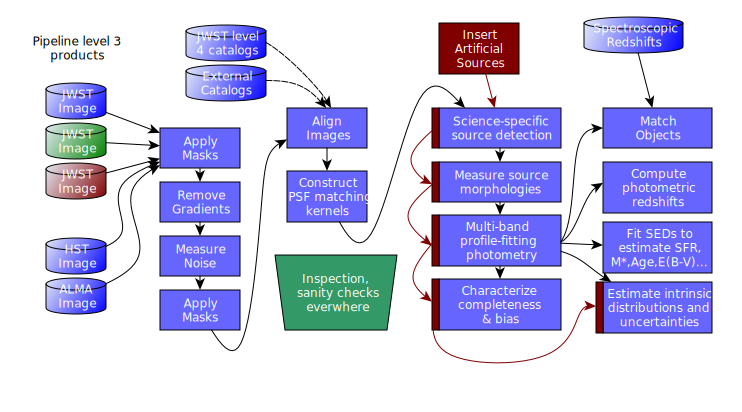
\includegraphics{faint_galaxy_photometry.png}
\caption{How does it flow?}\end{figure}

That was a flow diagram.


\chapter{Indices and tables}
\label{index:indices-and-tables}\label{index::doc}\begin{itemize}
\item {} 
\emph{genindex}

\item {} 
\emph{modindex}

\item {} 
\emph{search}

\end{itemize}



\renewcommand{\indexname}{Index}
\printindex
\end{document}
